\section{Independent Random Variables}

But, wait!
There's more fun to be had with the coin and the die.
Let's take our two boxes and screw them together.
\begin{center}
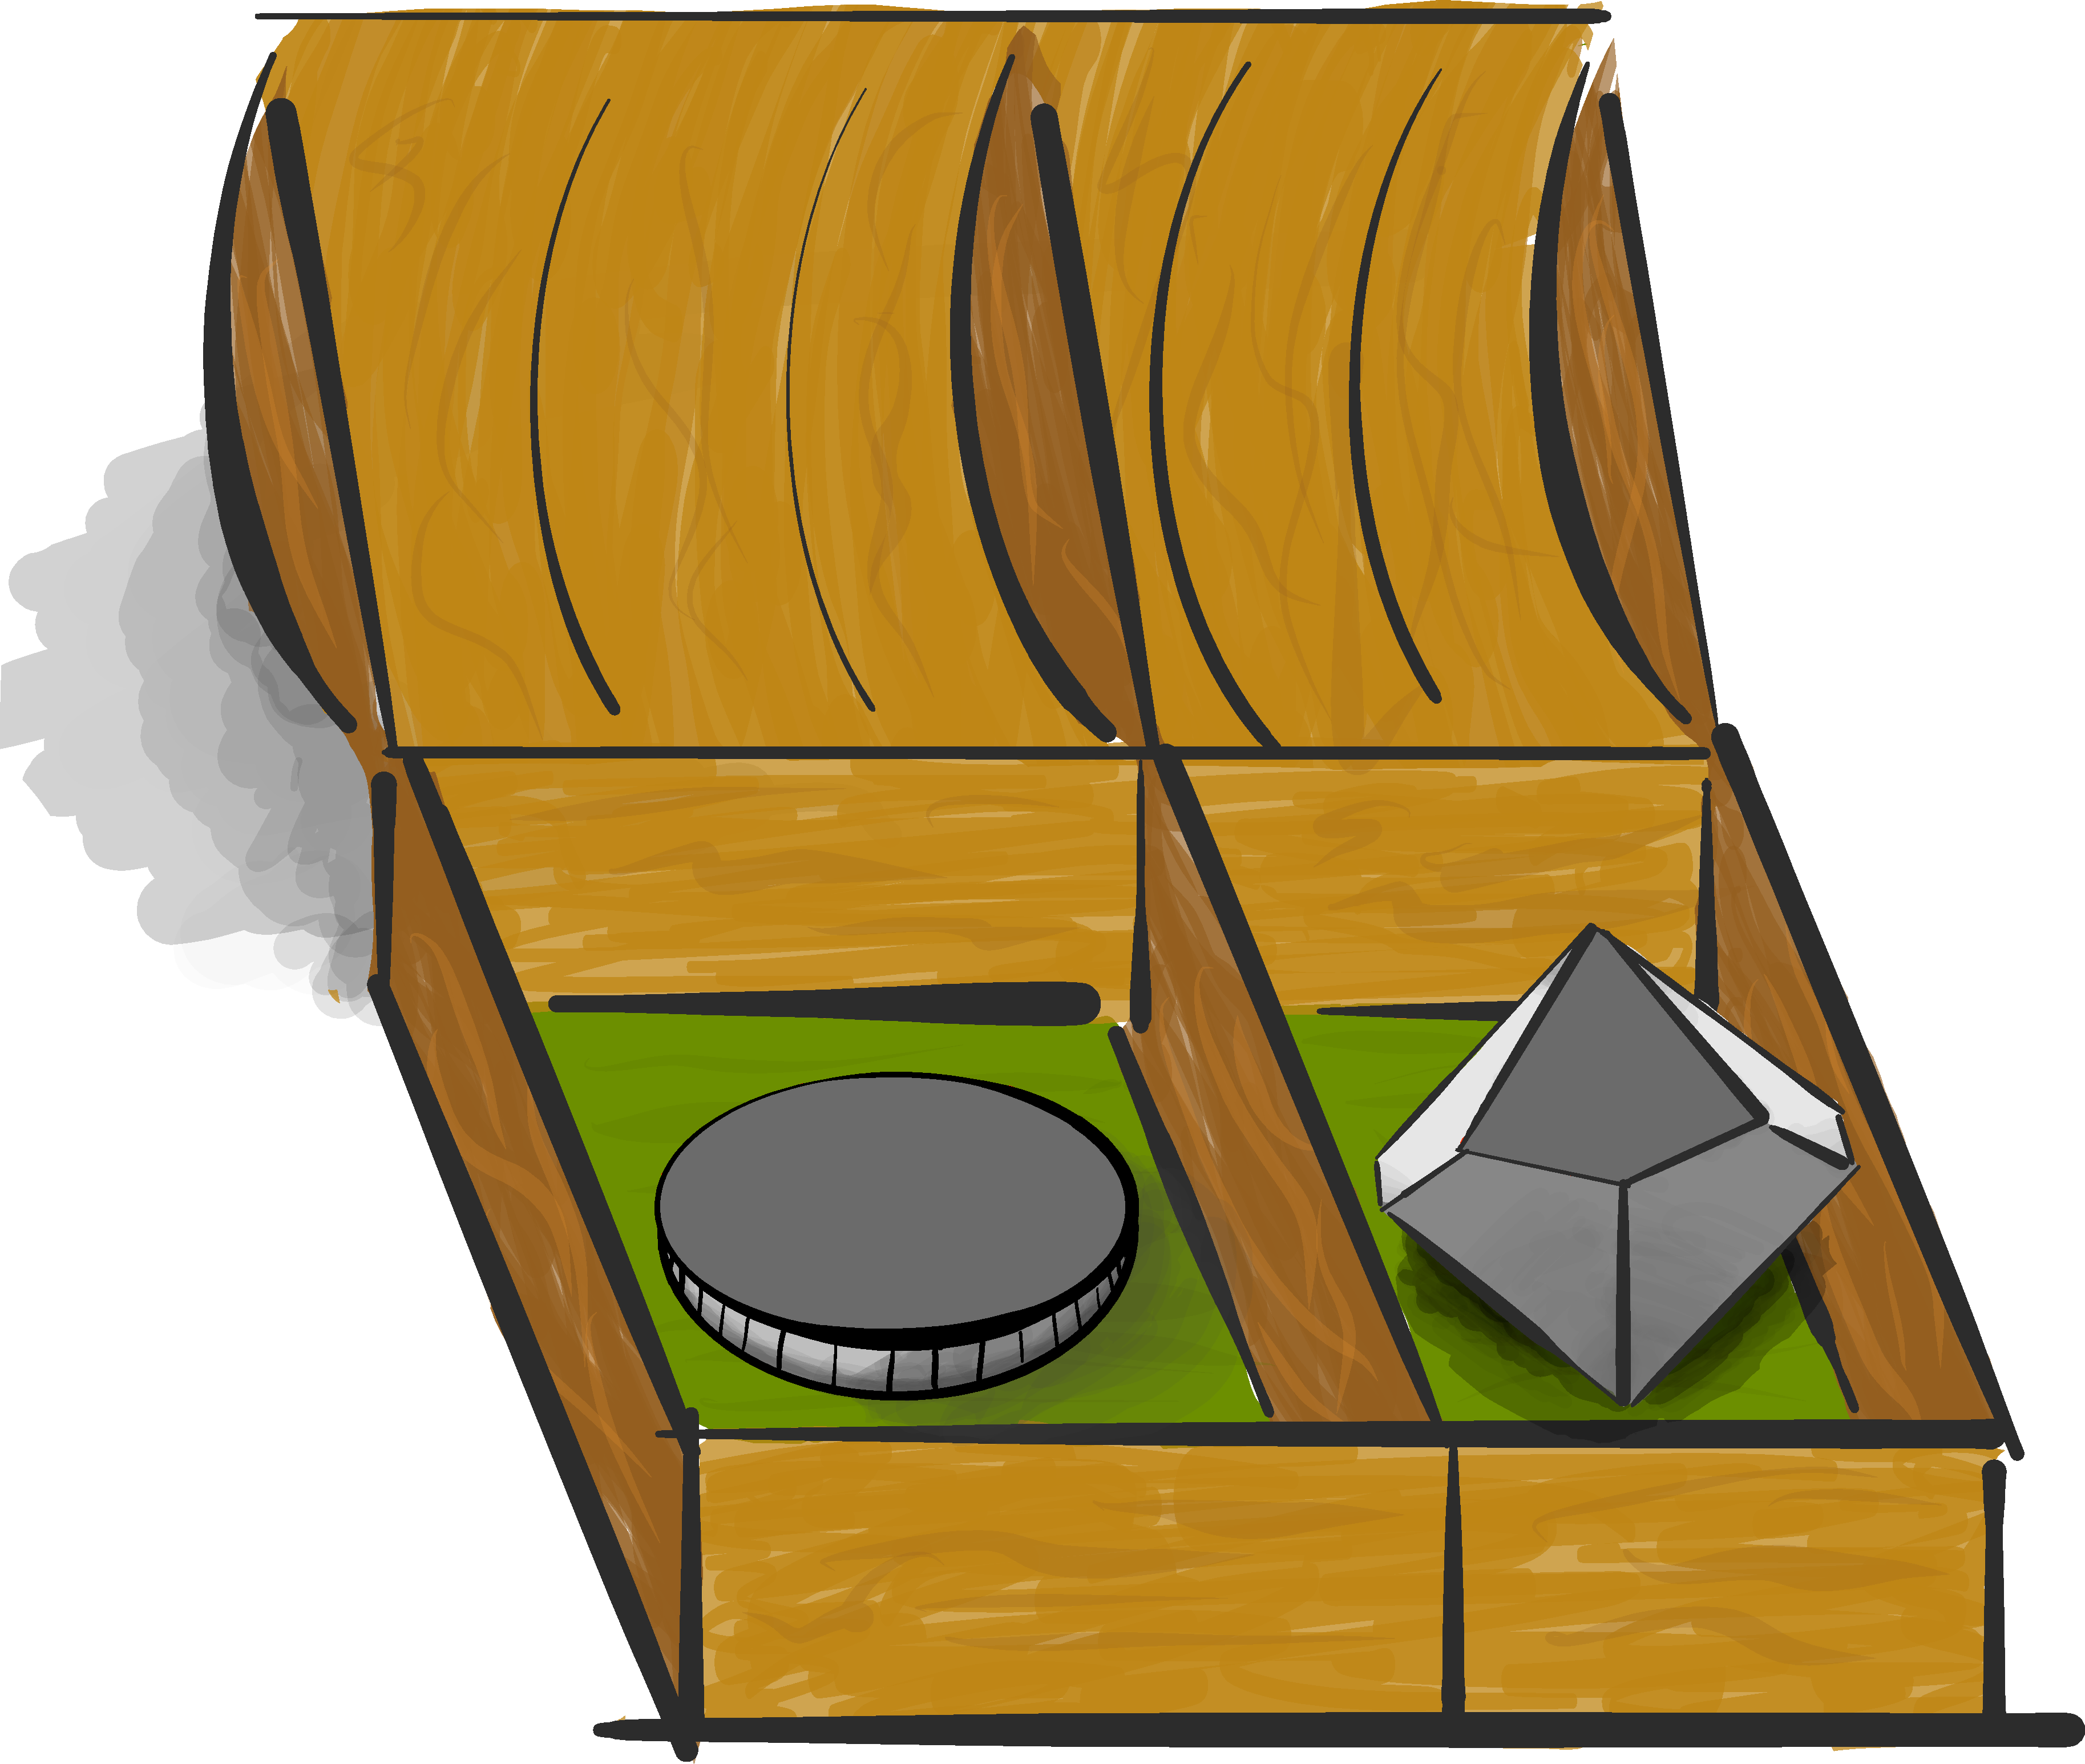
\includegraphics[width=0.4\textwidth]{img/box-both-open-coin-die}
\end{center}
As before, let's close both lids and give the big box a shake.
\begin{center}
\includegraphics[width=\textwidth]{img/both-box-closed-portal}
\end{center}
We will model the big box as a single random variable $\bm{A}$.
Now, there are four possible states that our big box could be in.
Both the coin and the die could be red side up or grey side up.
The possible states of the big box are summarized below.
\begin{center}
 \begin{tabular}{c c || c | c }
 \multicolumn{2}{c}{\multirow{2}{*}{$\bm{A}$}} & \multicolumn{2}{c}{$\bm{C}$} \\
\multicolumn{2}{c}{} & red & grey \\ [0.5ex]
 \hline\hline
\multirow{14}{*}{$\bm{D}$} & red
& \makecell{
  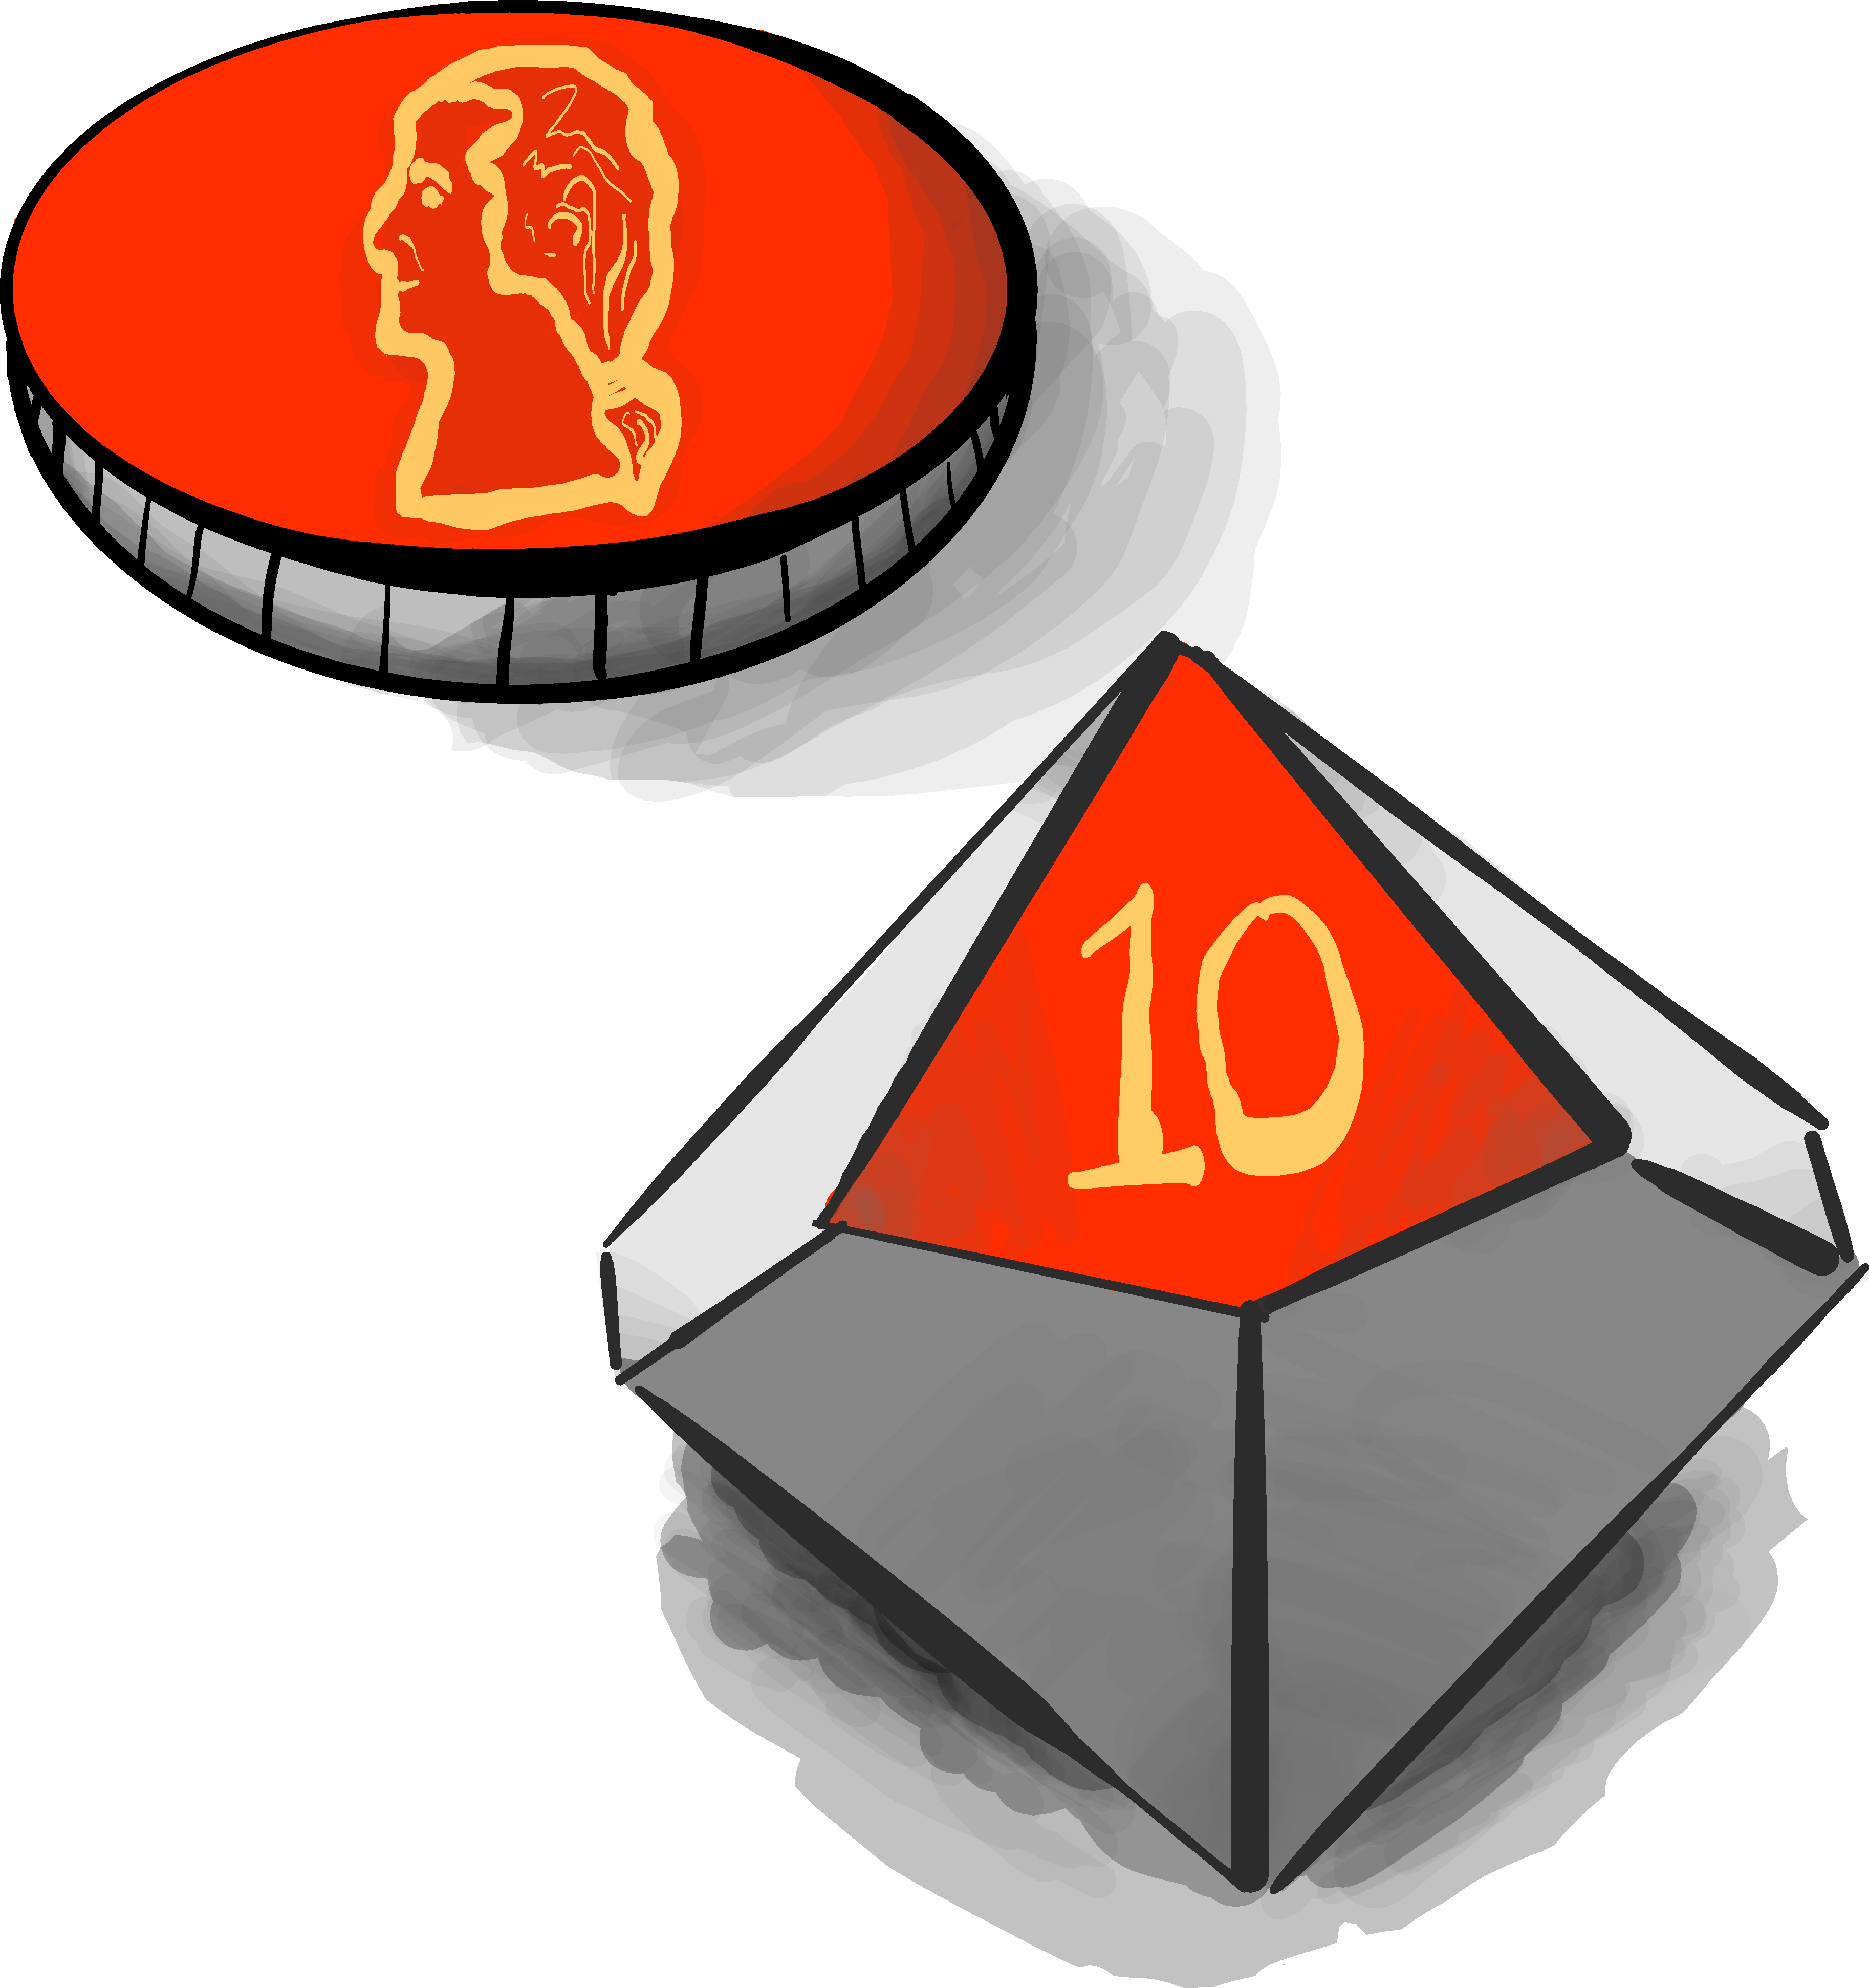
\includegraphics[trim= 0 0 0 -20ex, clip, width=0.3\textwidth]{img/red-coin-red-die} \\
  $\bm{A} = \text{``red coin, red die''}$
  }
 & \makecell{
  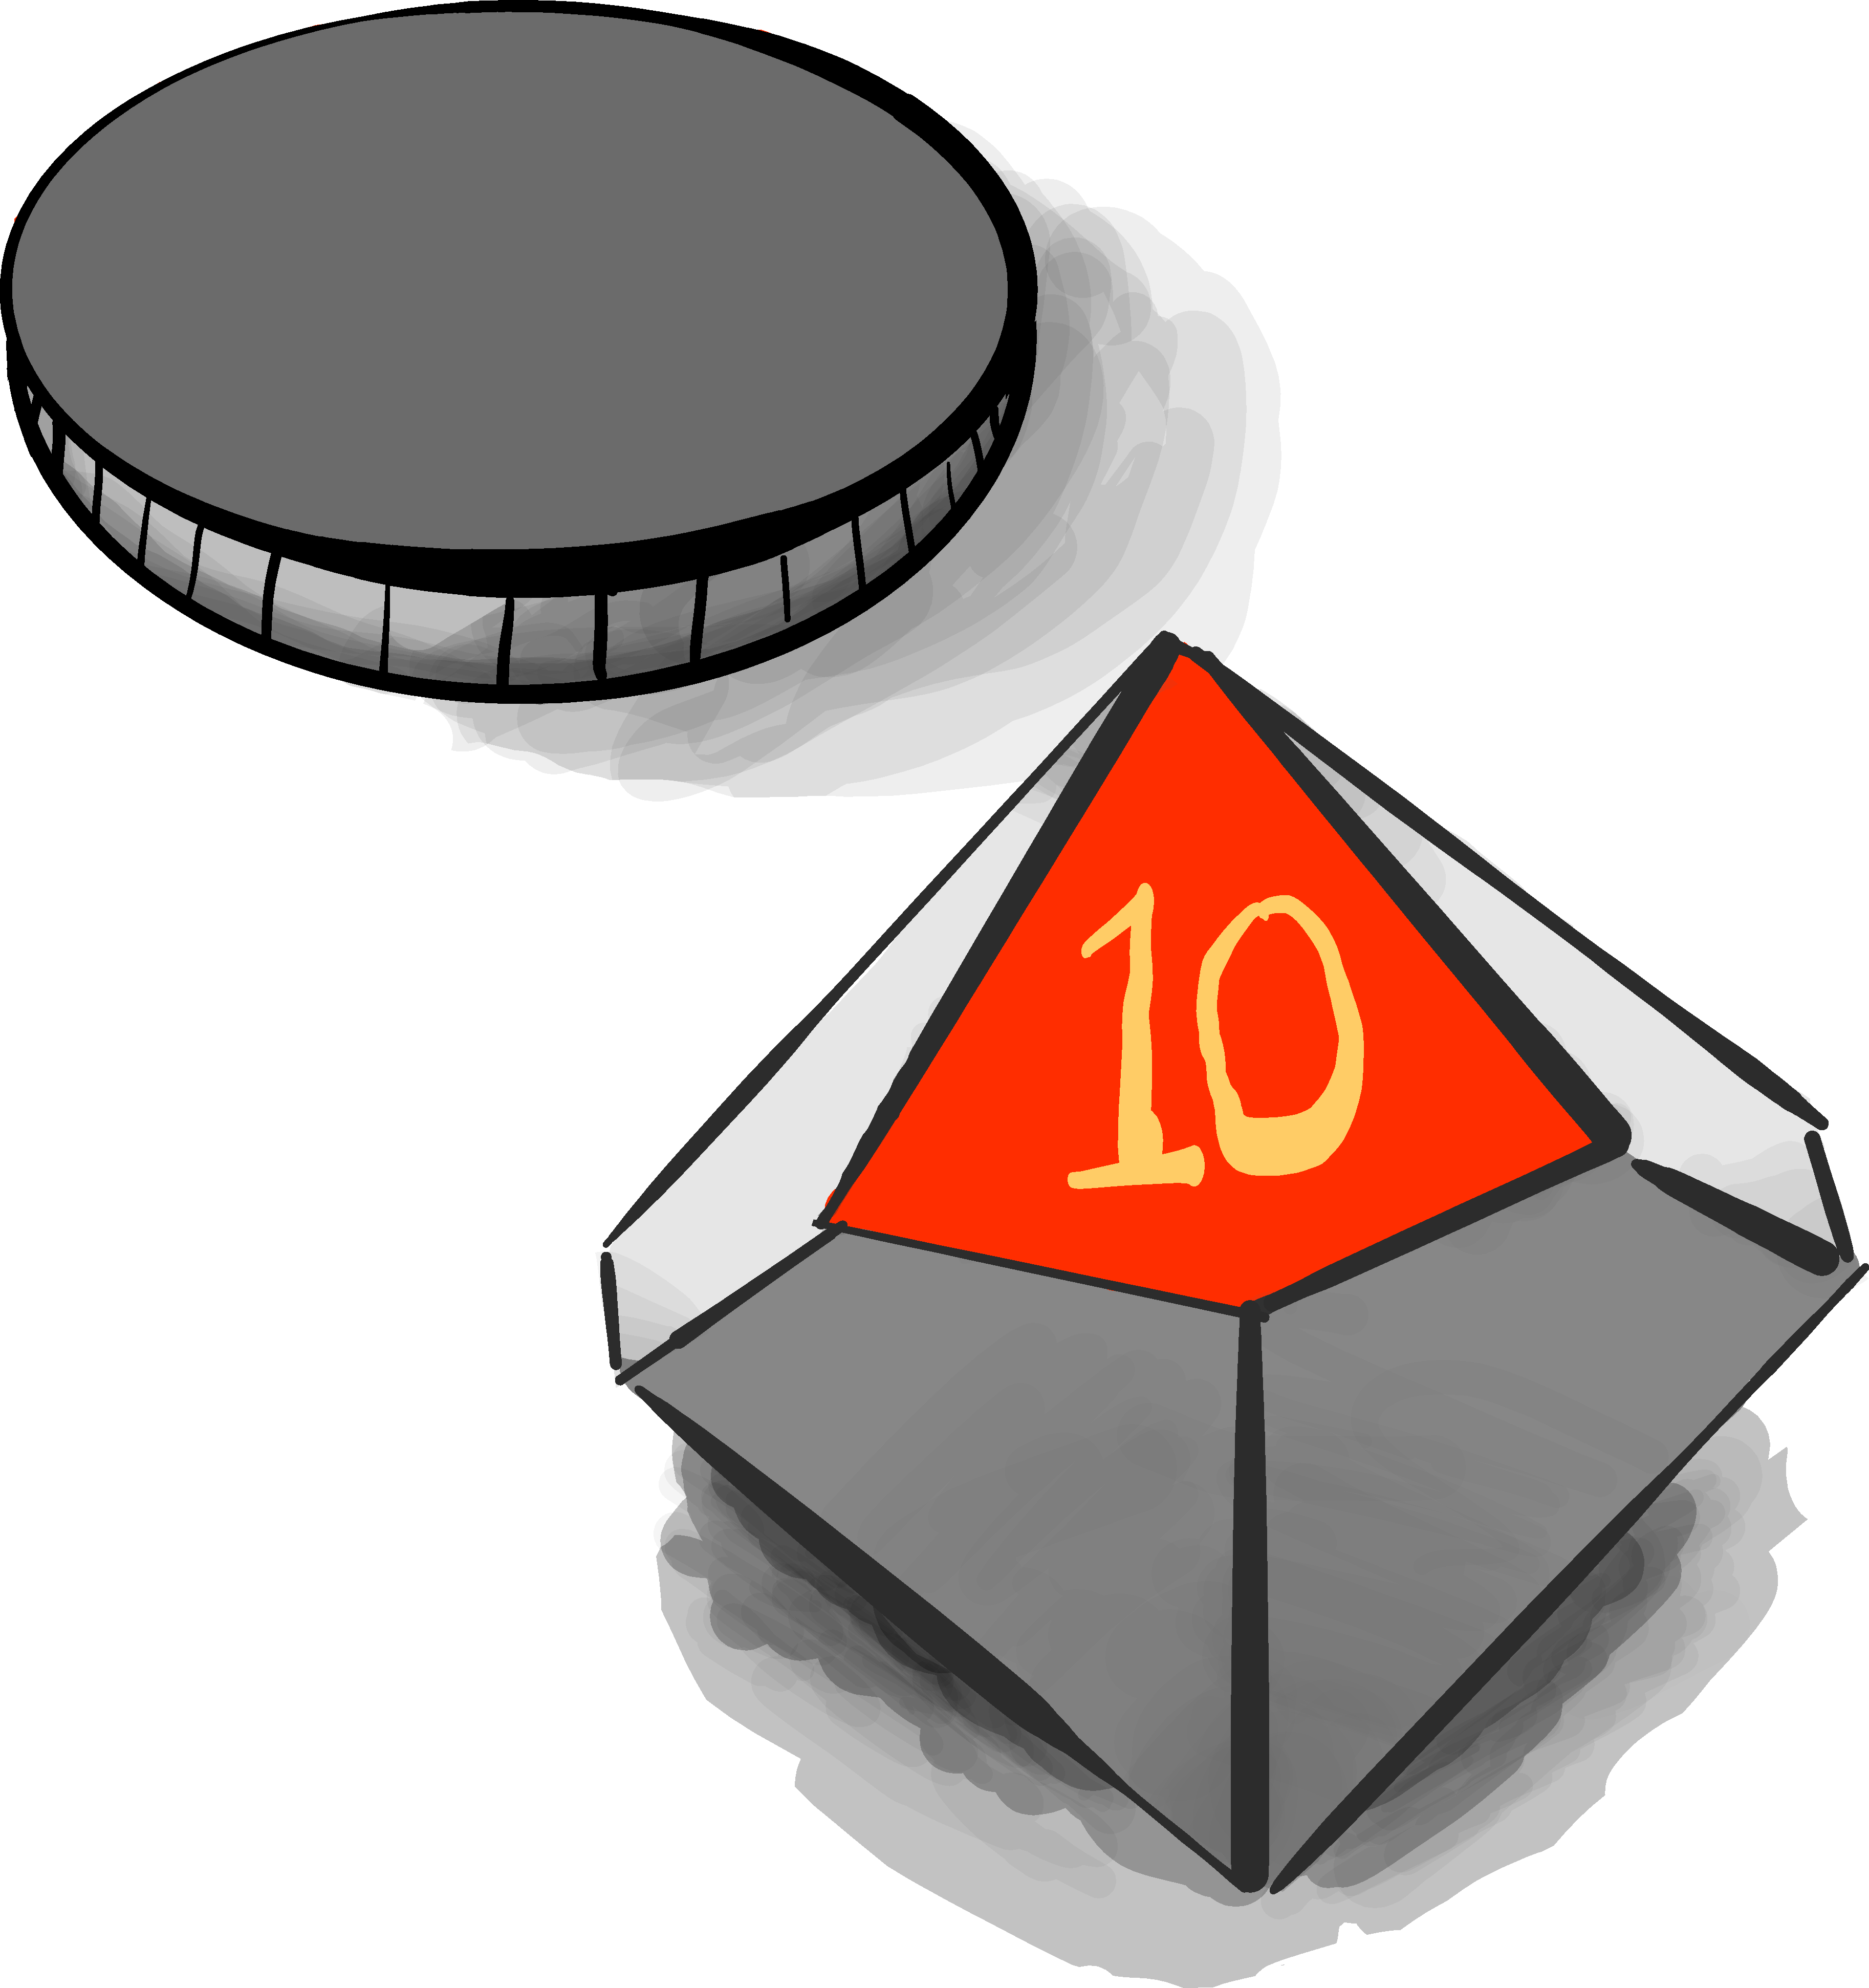
\includegraphics[trim= 0 0 0 -20ex, clip, width=0.3\textwidth]{img/grey-coin-red-die} \\
  $\bm{A} = \text{``grey coin, red die''}$
  }
  \\
 \cline{2-4}
 & grey
 & \makecell{
 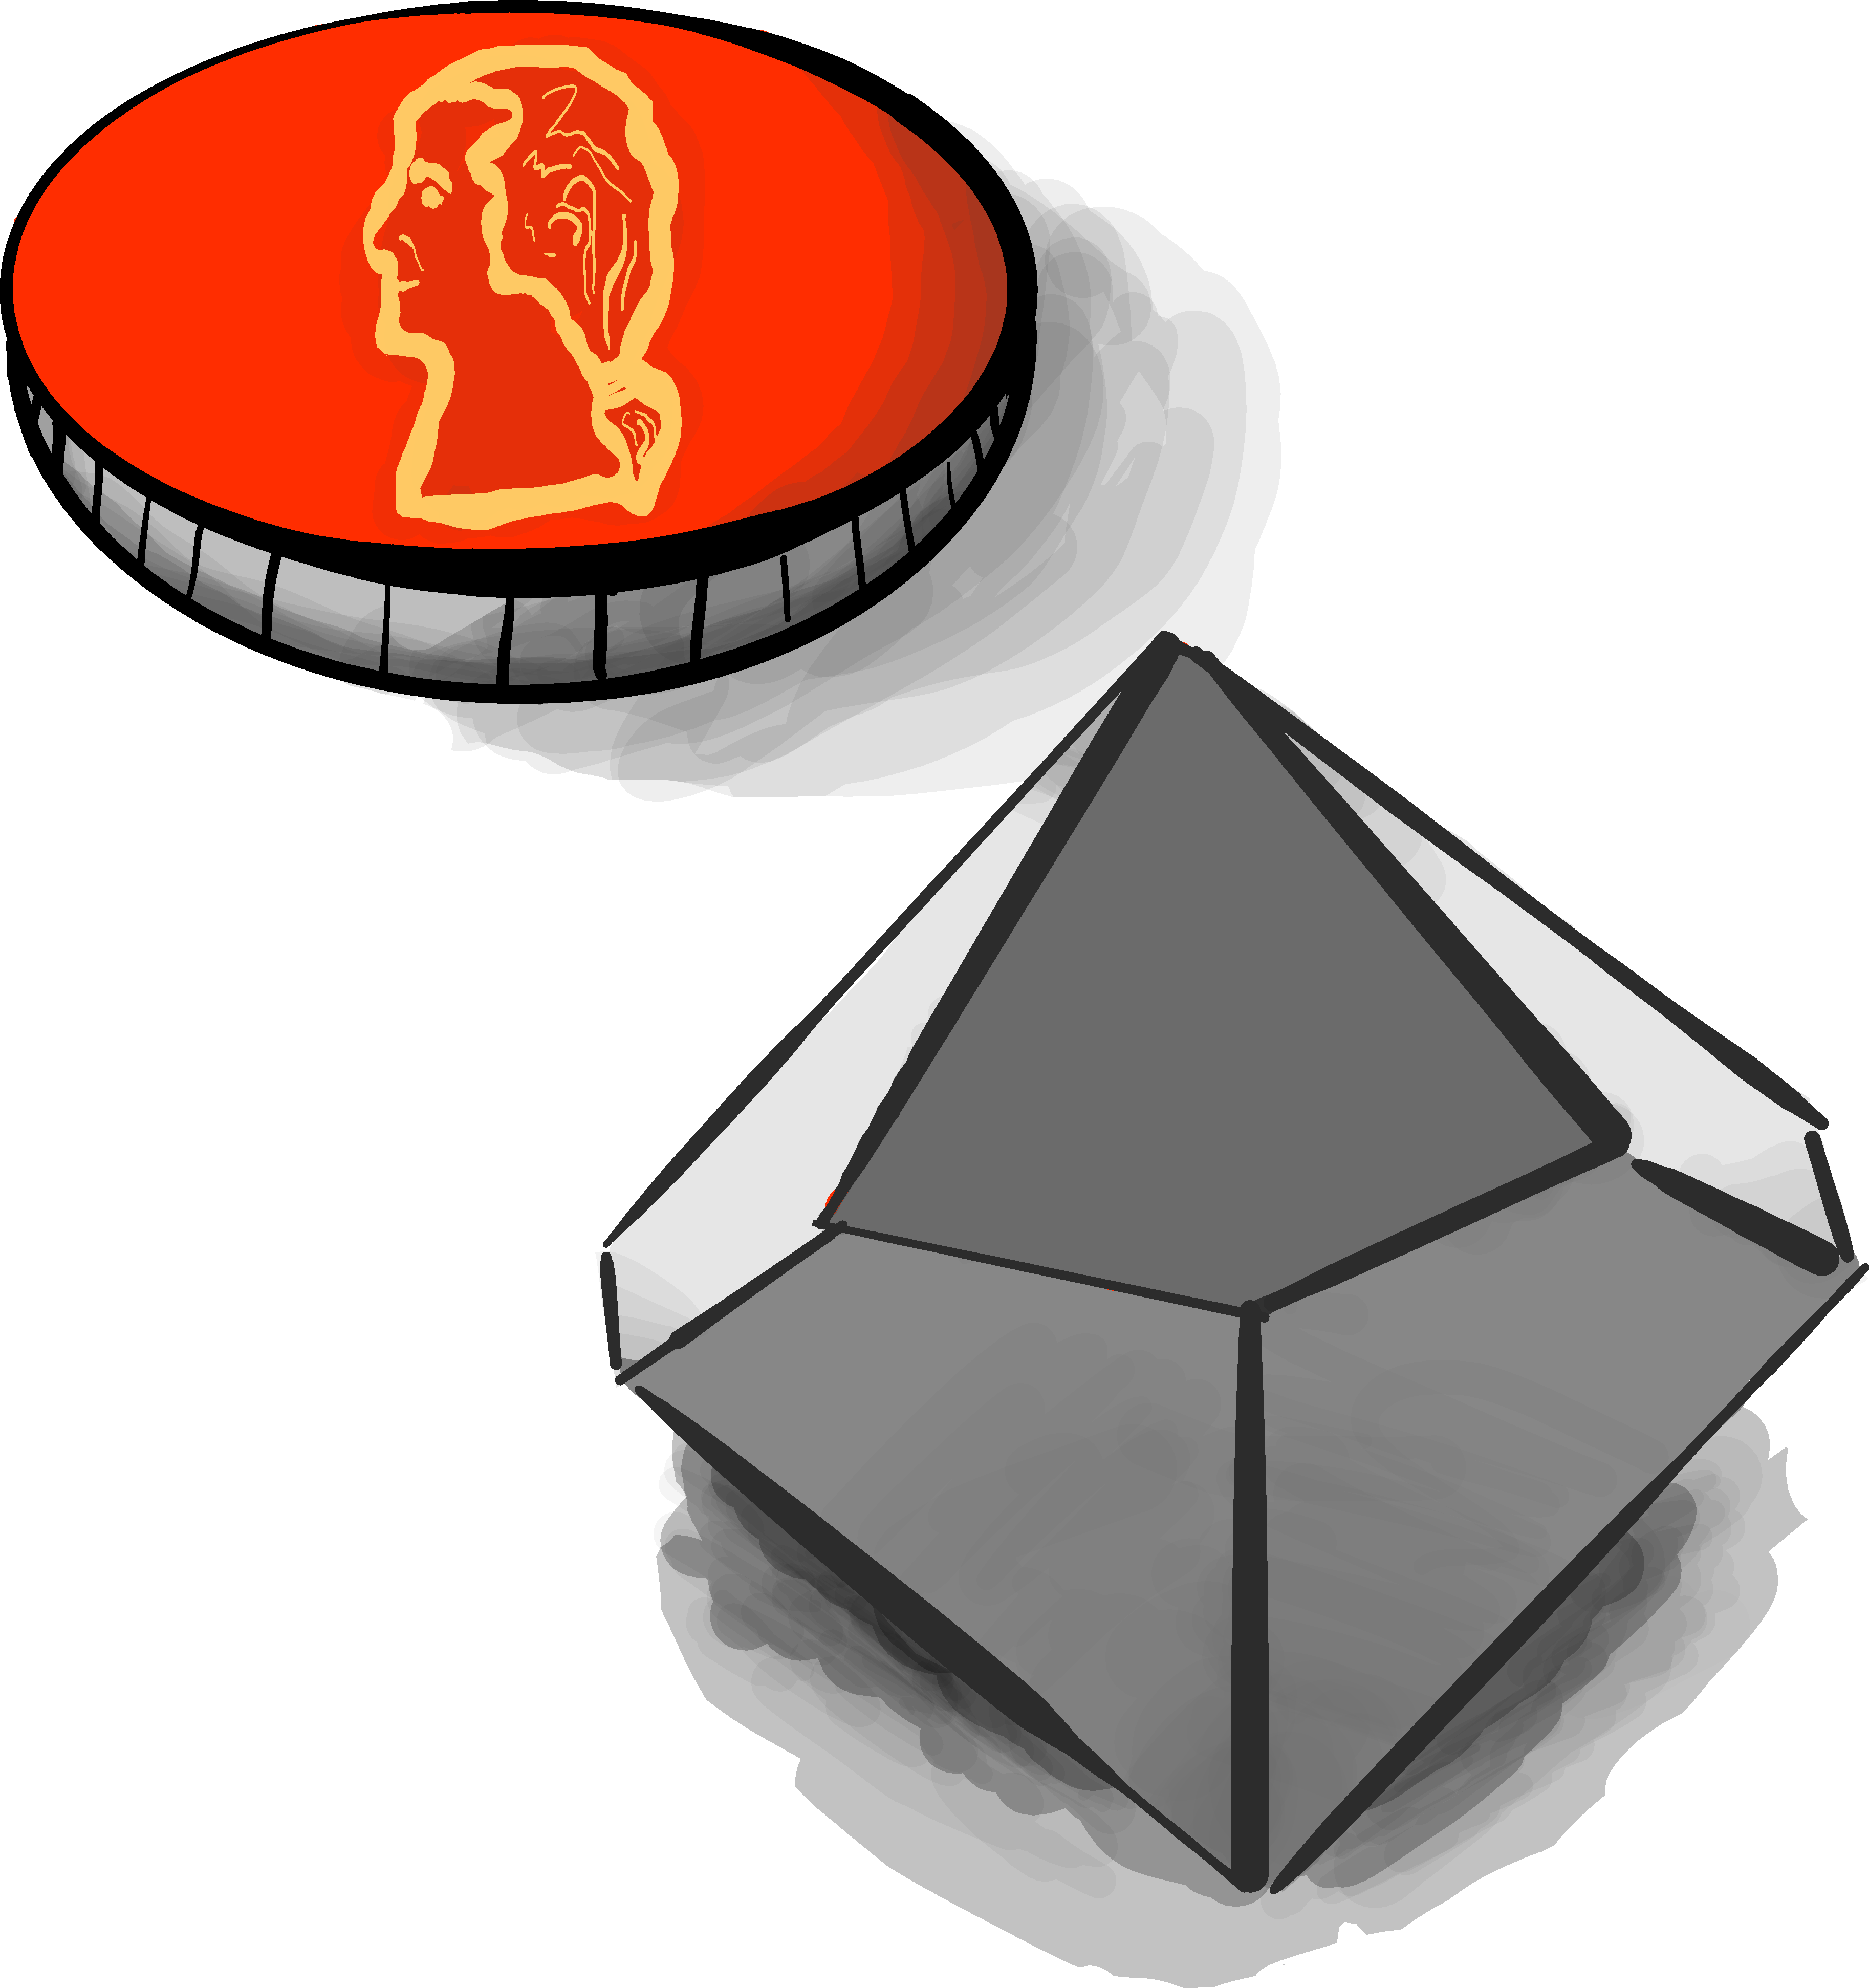
\includegraphics[trim= 0 0 0 -20ex, clip, width=0.3\textwidth]{img/red-coin-grey-die} \\
  $\bm{A} = \text{``red coin, grey die''}$}
 & \makecell{
 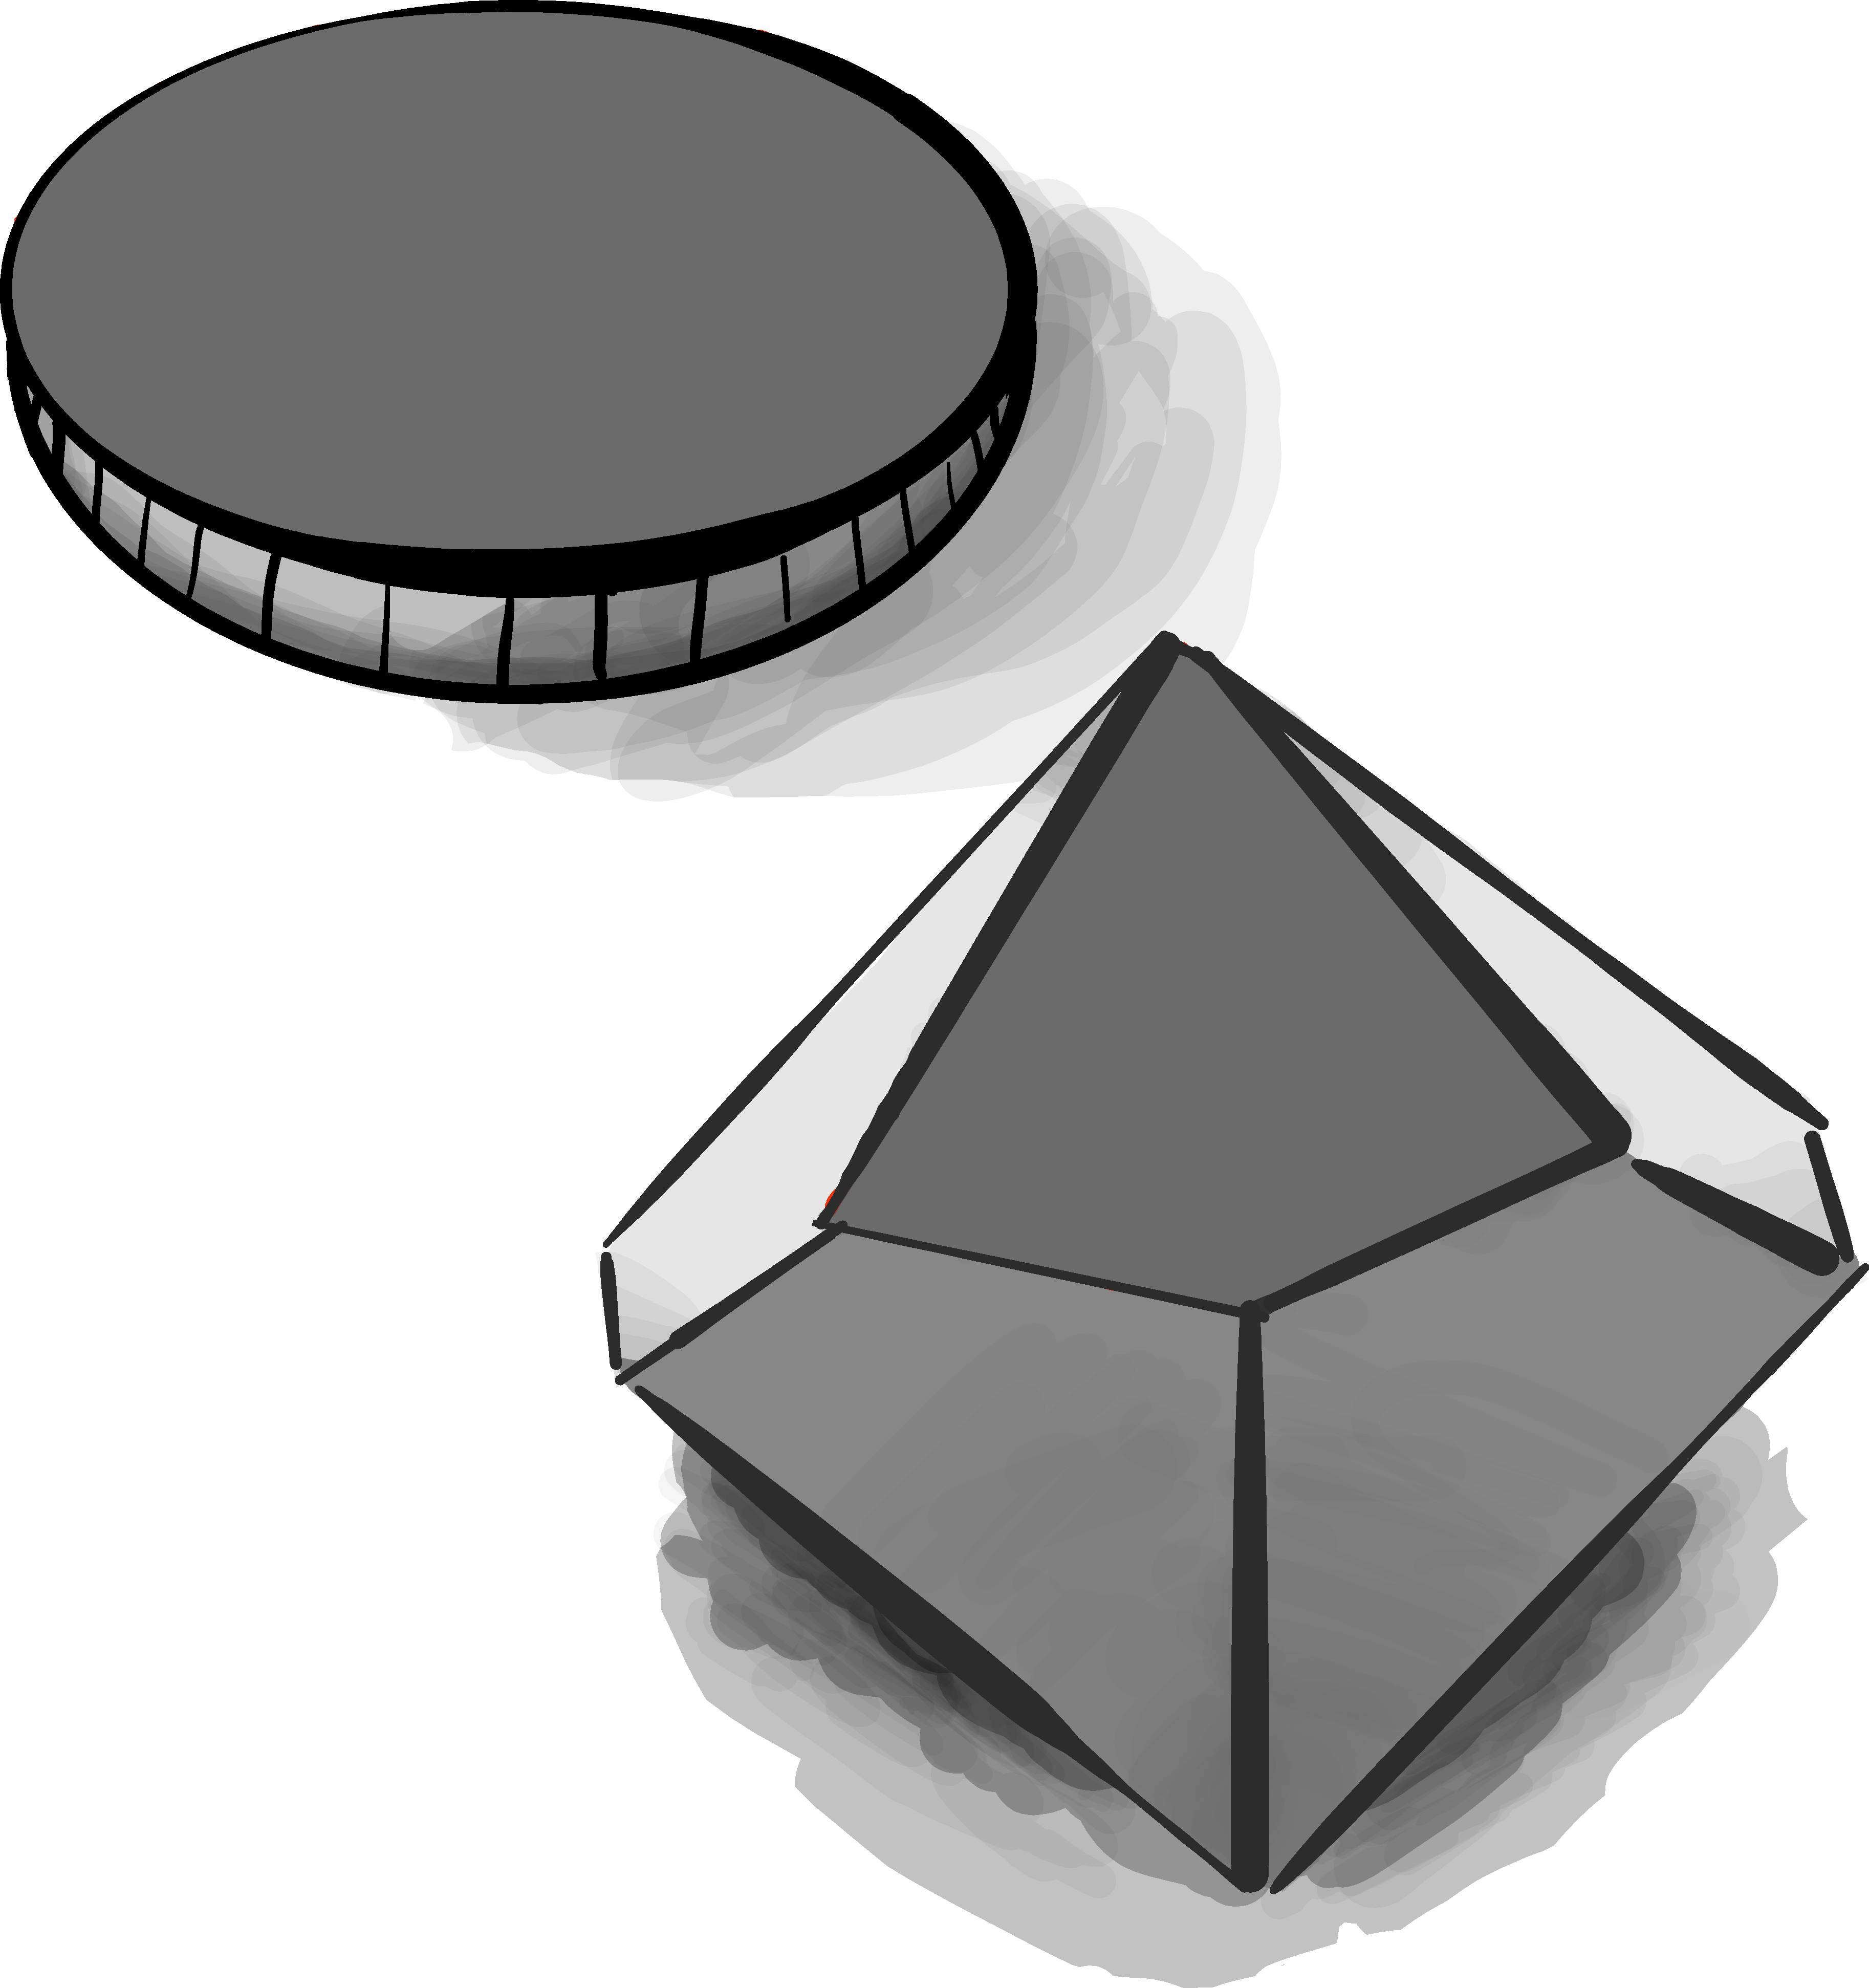
\includegraphics[trim= 0 0 0 -20ex, clip, width=0.3\textwidth]{img/grey-coin-grey-die} \\ $\bm{A} = \text{``grey coin, grey die''}$}
\end{tabular}
\end{center}

Because the die and the coin are independent, it is straightforward to calculate the probability of each of the four possible states of the big box.
For example, to compute the probability that the die and the coin are both grey side up we calculate,
\begin{align*}
p_{\bm{A} = \text{``grey coin, grey die''}}
&= p_{\bm{C} = \text{grey}} \times p_{\bm{D} = \text{grey}} \\
&= 0.5 \times 0.9 \\
&= 0.45.
\end{align*}
The probabilities of all four possible states of the big box are summarized below.
\begin{center}
 \begin{tabular}{c c || c | c || c}
 \multicolumn{2}{c}{\multirow{2}{*}{$\bm{A}$}} & \multicolumn{2}{c}{$\bm{C}$} & {}\\
\multicolumn{2}{c}{} & red & grey & sum \\ [0.5ex]
 \hline\hline
\multirow{2}{*}{$\bm{D}$} & red & 0.05 & 0.05 & 0.1 \\
 \cline{2-5}
 & grey & 0.45 & 0.45 & 0.9 \\
 \hline\hline
  {} & sum & 0.5 & 0.5 & 1 \\ [1ex]
\end{tabular}
\end{center}

Now that we know the probabilities for all the possible outcomes of $\bm{A}$, we can calculate the entropy associated with the the closed box.
\begin{align*}
S_{\text{big box}}
&=
H(\bm{A}) \\
&=
- 0.05 \times \log_2(0.05)
+ - 0.05 \times \log_2(0.05)
- 0.45 \times \log_2(0.45)
+ - 0.45 \times \log_2(0.45) \\
\approx 1.469
\end{align*}

Let's take a moment to notice,
\begin{align*}
S_{\text{big box}}
&=
S_{\text{die}} + S_{\text{coin}}.
\end{align*}

Intuitively, it makes sense that the entropy associated with the big box is the same as the sum of the entropy associated with the die box and the entropy associated with the coin box.
This relation holds true because the coin and the die are independent.
Intuitively speaking, the coin and the die are independent because knowing the state of the coin doesn't the probability of outcomes from the die and vice versa.
\begin{center}
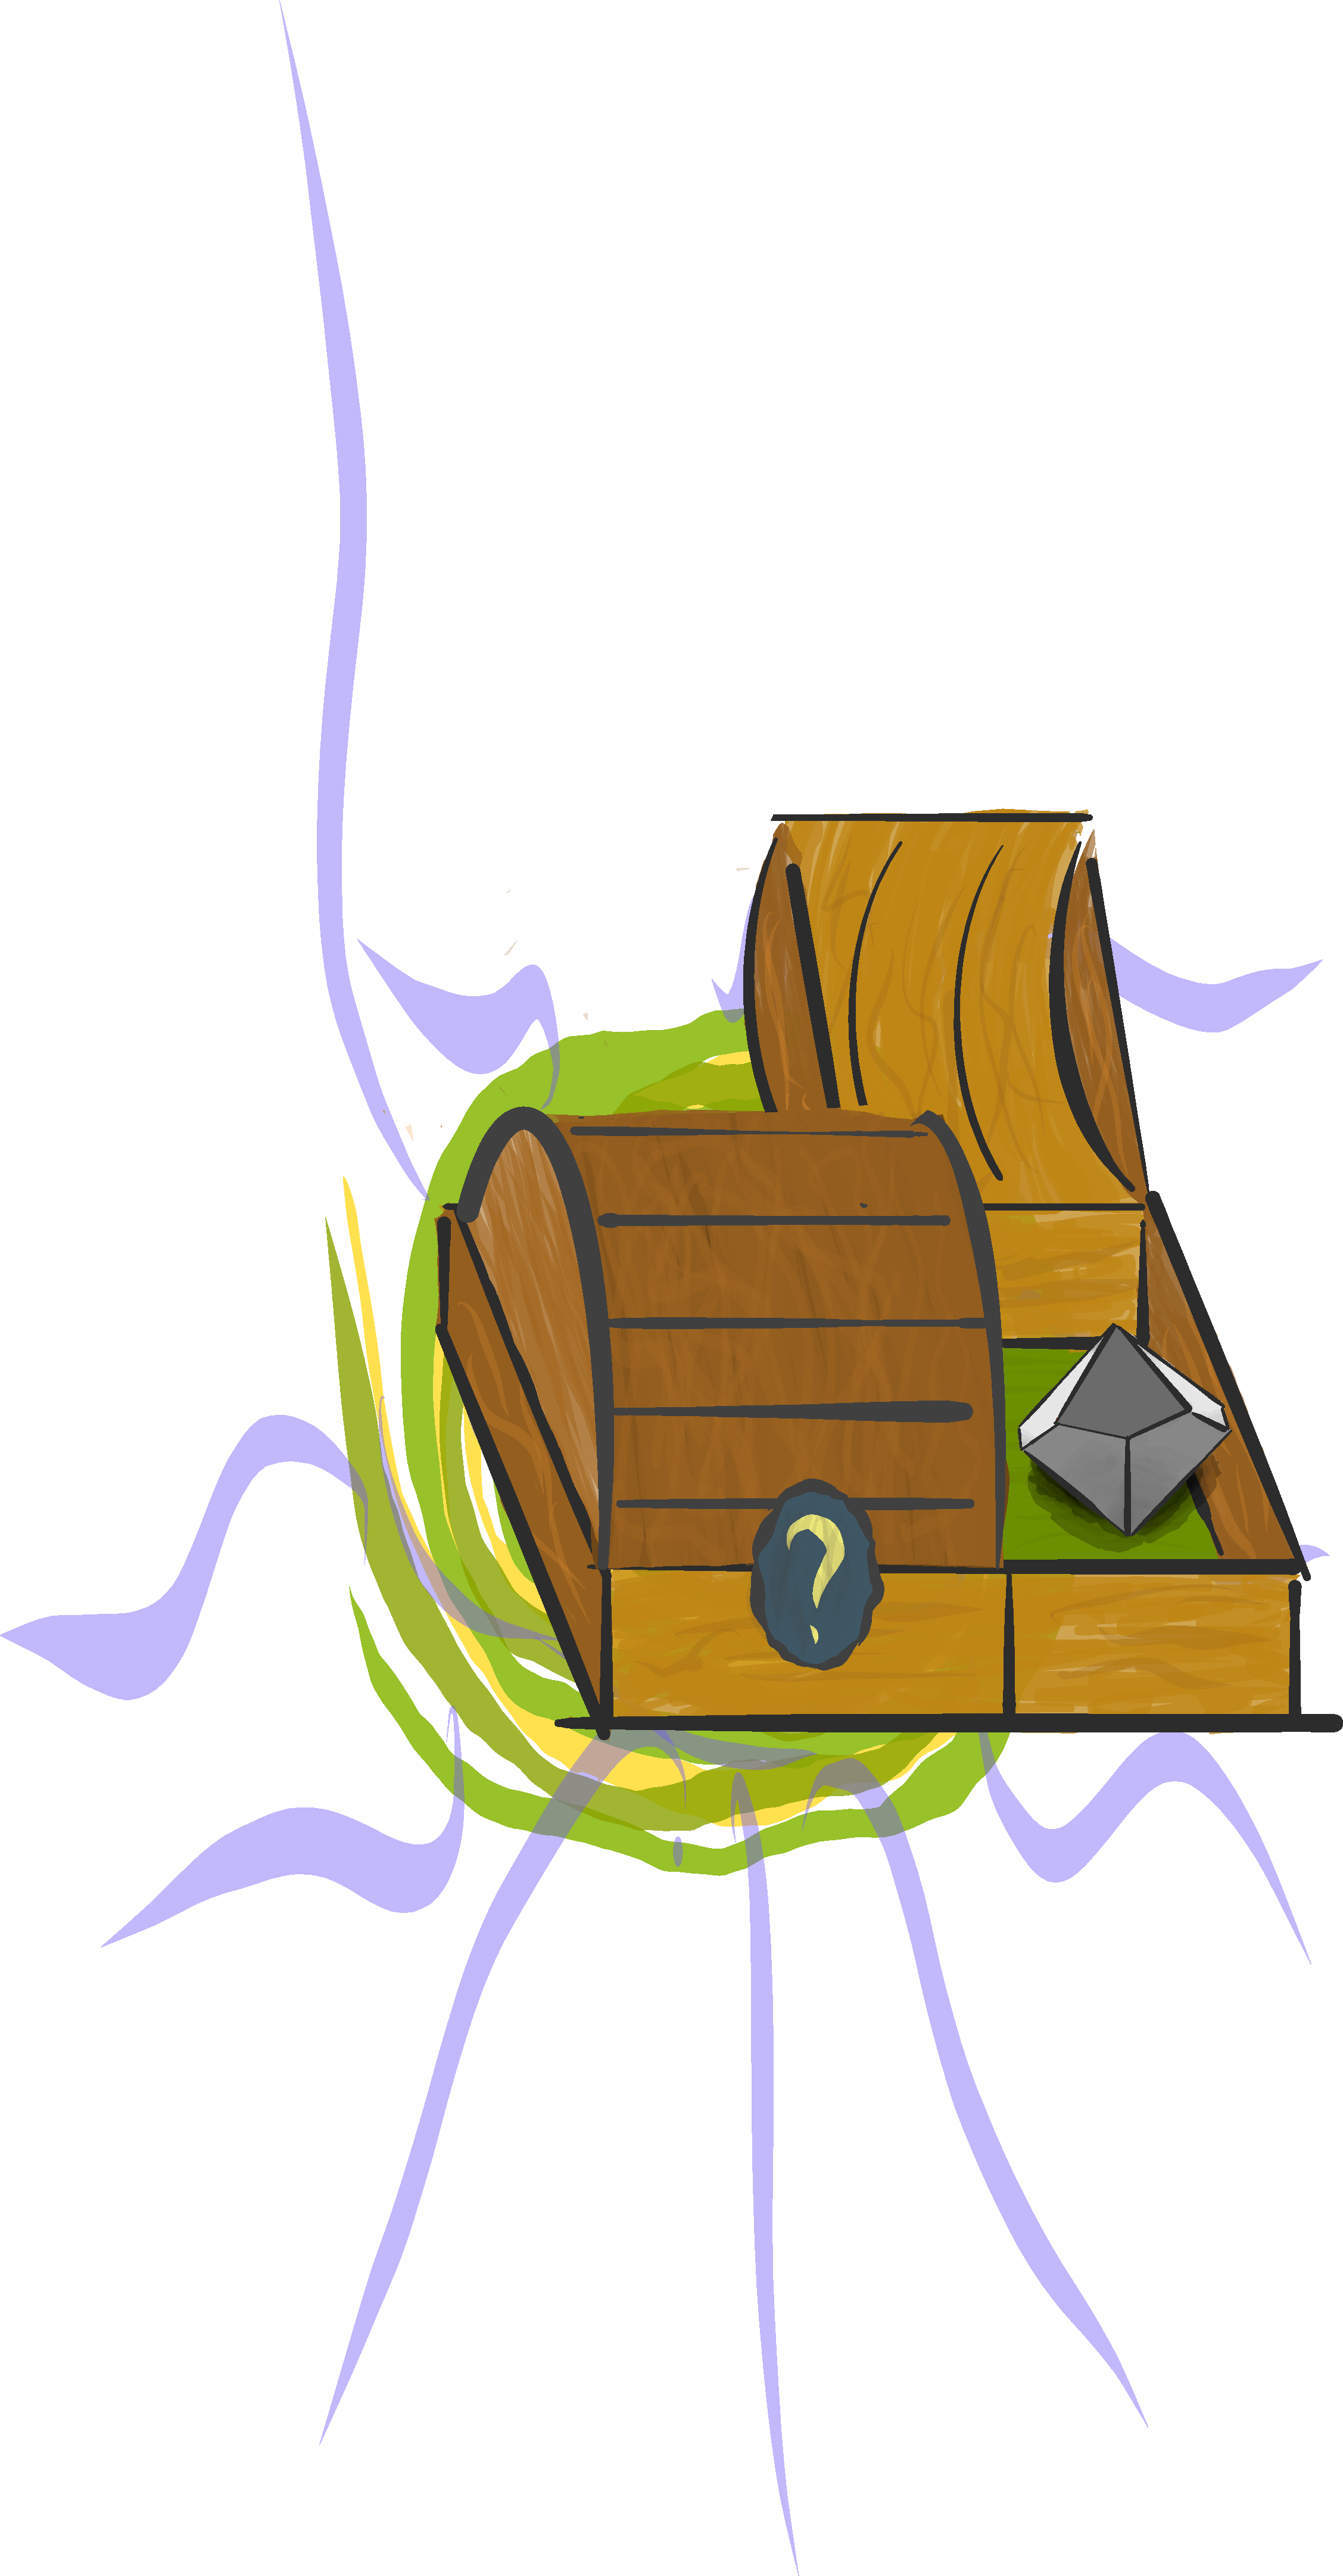
\includegraphics[width=0.3\textwidth]{img/left-box-closed-portal-die}
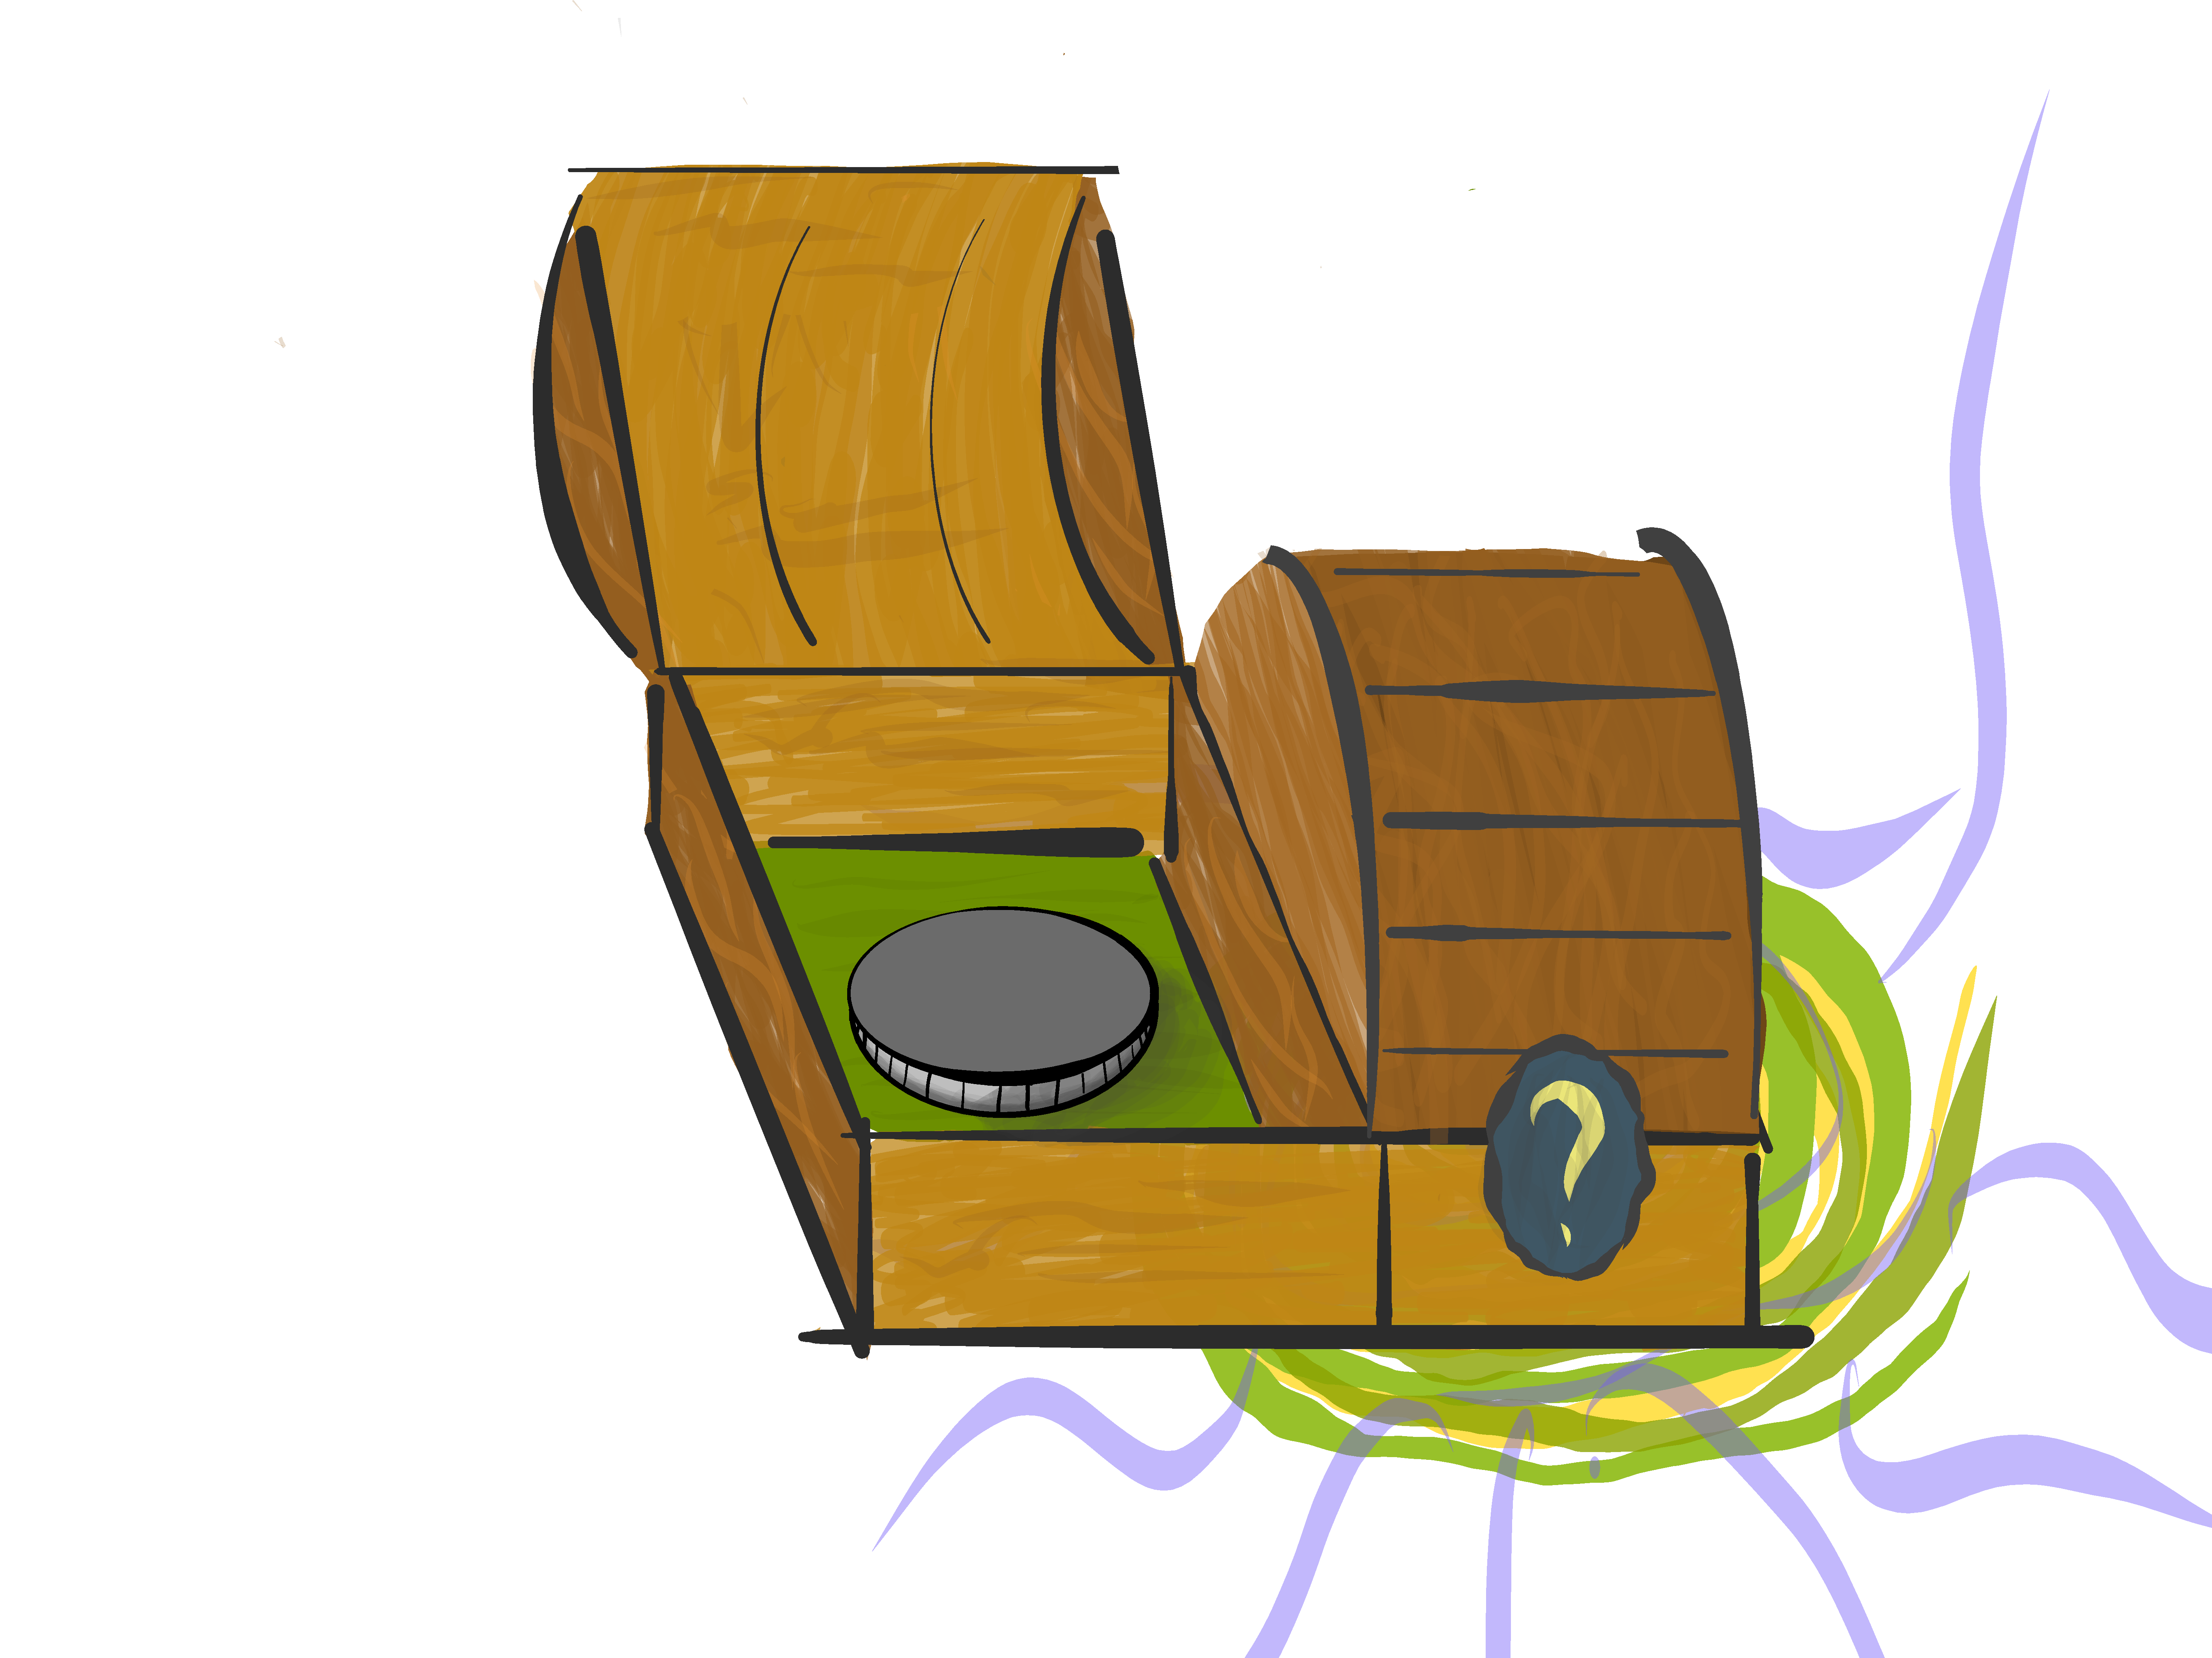
\includegraphics[trim= 0 -200ex 0 0, clip,width=0.4\textwidth]{img/right-box-closed-portal-coin}
\end{center}
The coin still has the same probability of taking on the red state or grey state given we know the state of the die.
The die still has the same probability of taking on the red state or grey state given we know the state of the coin.
Mathematically,
\begin{align*}
P(\bm{C}) &= P(\bm{C} | \bm{D}) \\
P(\bm{D}) &= P(\bm{D} | \bm{C}) .
\end{align*}
For those unfamiliar, the vertical bar is read as ``given.''

In the next section, we'll look at entropy and information in a situation where independence \textit{doesn't} hold.
This is where things get a little more interesting.
